\documentclass[conference]{IEEEtran}
\IEEEoverridecommandlockouts
% The preceding line is only needed to identify funding in the first footnote. If that is unneeded, please comment it out.
\usepackage{cite}
\usepackage{amsmath,amssymb,amsfonts,mathtools}
\usepackage{algorithmic}
\usepackage{graphicx}
\usepackage{textcomp}
\usepackage{xcolor}
\usepackage{indentfirst}
\usepackage{hyperref}
\hypersetup{
    colorlinks=true,
    linkcolor=blue,
    filecolor=magenta,      
    urlcolor=cyan,
}
\def\BibTeX{{\rm B\kern-.05em{\sc i\kern-.025em b}\kern-.08em
    T\kern-.1667em\lower.7ex\hbox{E}\kern-.125emX}}
\begin{document}

\title{To find Minimum Spanning Tree using Prim's Algorithm\\
{\footnotesize \textsuperscript {} Indian Institute of Information Technology, Allahabad}
}

\author{\IEEEauthorblockN{Aditya Aggarwal}
\IEEEauthorblockA{\textit{iit2019210@iiita.ac.in}}
\and
\IEEEauthorblockN{Divy Agrawal}
\IEEEauthorblockA{\textit{iit2019211@iiita.ac.in}}
\and
\IEEEauthorblockN{Aman Rubey}
\IEEEauthorblockA{\textit{iit2019212@iiita.ac.in}}
}

\maketitle

\begin{abstract}
 In this paper we will use Prim's Algorithm to find the Minimum Spanning Tree. Also in the later part of the paper we have discussed the space and time complexity of the devised algorithm.
\end{abstract}

\begin{IEEEkeywords}
Algorithm, Graph's, Minimum Spanning Tree, Prim's Algorithm, Complexity
\end{IEEEkeywords}

\section{Introduction}
Prim's algorithm is a greedy algorithm that finds a minimum spanning tree for a weighted undirected graph. This means it finds a subset of the edges that forms a tree that includes every vertex, where the total weight of all the edges in the tree is minimized. 

\section{Algorithm Design}
We have been given a weighted graph by the user whose MST(minimum spanning tree) we have to find. The following steps will help us to find the MST for a given graph.
\begin{enumerate}
\item Create a boolean flag array(initialized to false) which has size as number of vertices which will be used to track that which vertex is taken for MST and which not.
\item Create another vector namely, ‘min\_weight’ of same size where we will store the weight of the minimum weighted edge its connected to, such that the other endpoint of the edge is already taken in flag array.
\item Consider any vertex as the starting node and so flag[start\_node] will be made true as starting node is included in MST and also min\_weight for it will 0.
\item Now, iterate for (vertices-1) times and in every iteration follow next steps:
\begin{enumerate}
    \item Get the the minimum weighted index or (u).
    \item A minimum weighted index is that index for which the corresponding vertex is not taken and also it has minimum key in the min\_weight vector.
    \item Include u to flag array.
    \item For every v in V update the min\_weight , where V is set of all vertices for which graph(u, v)>0.
    \item To update min\_weight for ‘v’: if graph(u,v)\ <\ min\_weight[v] then min\_weight[v]=graph(u,v)
    \item Here graph is a vector which is used to store the original graph in the form of adjacency matrix.
\end{enumerate}
\end{enumerate}
After performing the above steps the Tree obtained will be a MST.
\section{Pseudo Code}
\vspace{5pt}
\hrule height 0.4pt depth 1pt width 250pt \relax
\vspace{5pt}
\textbf{MST using Prim's Algorithm}
\vspace{5pt}
\hrule height 0.4pt depth 1pt width 250pt \relax
\vspace{5pt}
\textbf{\textit{Global Variables:}}\\
\hspace*{7mm} int\ vertices;\\
\\
\hspace*{4mm}\textbf{\textit{function}}\ main()\\
\hspace*{7mm}Get\ number\ of\ vertices;\\
\hspace*{7mm}Get\ the\ edges\ in\ form\ of\ u\ v\ weight(u,v);\\
\hspace*{7mm}store\ the\ edges\ in form\ adjacency\ matrix;\\
\hspace*{7mm}graph[u-1][v-1]\ \leftarrow\ weight;\\
\hspace*{7mm}graph[v-1][u-1]\ \leftarrow\ weight;\\
\hspace*{7mm}call\ Prim\_Min\_spanning\_Tree\ function;\\
\hspace*{7mm}return\ 0;\\
\\
\hspace*{4mm}\textbf{\textit{function}}\ Prim\_Min\_spanning\_Tree(adjacency\ matrix\ graph)\\
\hspace*{7mm}Define\ vector\ of\ int\ min\_spanning\_tree(vertices)\\
\hspace*{7mm}Define\ vector\ of\ int\ min\_weight(vertices)\\
\hspace*{7mm}Define\ vector\ of\ bool\ flag(vertices)\\
\hspace*{7mm}As\ there\ will\ be\ no\ edges\ in\ MST\ so\\
\hspace*{7mm}min\_weight\ will\ be\ initialized\ as\ INT\_MAX\\
\hspace*{7mm}flag\ will\ be\ initialized\ as\ false\\
\hspace*{7mm}min\_weight[0]\ \leftarrow\ 0\\
\hspace*{7mm}min\_spanning\_tree[0]\ \leftarrow -1\\
\hspace*{7mm}for(int\ i=0;\ i<vertices-1;\ i++)\\
\hspace*{10mm}int\ u\ =\ getMinWeight(min\_weight,\ flag);\\
\hspace*{10mm}flag[u]\ =\ true;\\
\hspace*{10mm}for(int\ v=0;\ v<vertices;\ v++)\\
\hspace*{13mm}if\ (graph[u][v]\ and\ flag[v]\ ==\ false\\
\hspace*{17mm}and\ graph[u][v]\ <\ min\_weight[v])\\
\hspace*{16mm}min\_spanning\_tree[v]\ =\ u;\\
\hspace*{16mm}min\_weight[v]\ =\ graph[u][v];\\
\hspace*{13mm}endif\\
\hspace*{10mm}endfor\\
\hspace*{7mm}endfor\\
\hspace*{7mm}return\ min\_spanning\_tree\\
\\
\hspace*{4mm}\textbf{\textit{function}}\ getMinWeight(min\_weight,\ flag)\\
\hspace*{7mm}Find\ the\ vertex\ not\ visited\ yet\\
\hspace*{7mm}and\ having\ minimum\ value\ in\ min\_weight\\
\hspace*{7mm}return\ vertex\\
\vspace{5pt}
\hrule height 0.4pt depth 1pt width 250pt \relax
\vspace{5pt}
\section{Complexity Analysis}
In the next two sub-sections we analyse the time and space complexity of algorithm we devised for the given problem.
\subsection{Time-Complexity}
Let V denote the number of vertices in the given graph whose MST we have to find.\\
Taking  the reference of the above Pseudo Code, the outer for loop of the Prim\_Min\_spanning\_Tree function is running V times and the getMinWeight function is also running V times. Similarly the Inner for loop is also running V times.\\
Therefore,\\
\begin{equation}
    T(V) = O(V*(V+V)) + C\textsubscript{1}
\end{equation}
which is equivalent to,
\begin{equation}
    T(V) = O(2V\textsuperscript{2}) + \Theta(1)
\end{equation}
which is in turn equivalent to,
\begin{equation}
    T(V) = O(V\textsuperscript{2})
\end{equation}
\begin{figure}[htbp]
\centerline{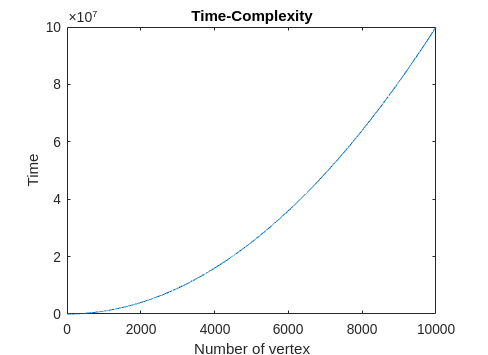
\includegraphics[width=8cm]{Time.png}}
\caption{Time–Complexity Graph (O(V\textsuperscript{2}))}
\label{fig}
\end{figure}
\\
\subsection{Auxiliary Space-Complexity}
Let V denote the number of vertices in the given graph whose MST we have to find.\\
Taking  the reference of the above Pseudo Code, we have created three vectors of size V mainly min\_weight, flag, min\_spanning\_tree.\\
Therefore,\\
\begin{equation}
    S(V) = O(3*V) + C\textsubscript{1}
\end{equation}
which is equivalent to,
\begin{equation}
    S(V) = O(V)
\end{equation}
\\
\begin{figure}[htbp]
\centerline{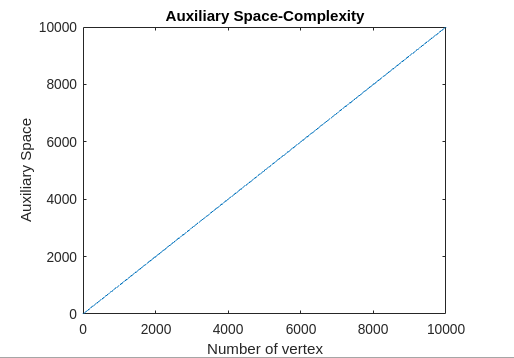
\includegraphics[width=8cm]{Space.png}}
\caption{Auxiliary Space–Complexity Graph (O(V))}
\label{fig}
\end{figure}
\section{Conclusion}
Therefore, using the concept of Prim's Algorithm we can find the Minimum Spanning Tree of a given graph in O(V\textsuperscript{2}) time and O(V) auxiliary space.\\
\begin{thebibliography}{00}
\bibitem{b1}Introduction to Algorithms 3rd Edition by Clifford Stein, Thomas H. Cormen, Charles E. Leiserson, Ronald L. Rivest
\bibitem{b2} Algorithm Design by J Kleinberg and E Tardos
\bibitem{b3}\href{https://en.wikipedia.org/wiki/Prim\%27s_algorithm}{Prim's Algorithm}
\bibitem{b4}\href{https://stackoverflow.com/questions/11032015/how-to-find-time-complexity-of-an-algorithm}{Complexity Analysis}
\bibitem{b5}\href{https://www.overleaf.com/latex/templates/ieee-conference-template-example/nsncsyjfmpxy}{IEEE Paper}
\end{thebibliography}
\end{document}